\uuid{mkeZ}
\exo7id{7601}
\auteur{mourougane}
\datecreate{2021-08-10}
\isIndication{false}
\isCorrection{true}
\chapitre{Autre}
\sousChapitre{Autre}

\contenu{
\texte{

}
\begin{enumerate}
    \item \question{Rappeler la définition de la branche principale du logarithme.}
\reponse{On définit une détermination du logarithme en posant
$$\begin{array}{cccc}
 l_+ :& \Cc-]-\infty,0] & \longrightarrow & \Cc\\ & z=re^{i\theta} (r>0, -\pi<\theta<\pi)&\longmapsto& \log_\Rr(r)+i\theta.
\end{array}$$
C'est une application continue, et même holomorphe telle que $$\forall z\in\Cc-]-\infty,0],\ \ e^{l_+(z)}=z.$$}
    \item \question{Peut on définir un logarithme sur $\Cc-C$ le plan complexe privé de l'ensemble
$$ C:= [ \; 0,1\; ] \cup \{ \; z \in \mathbb{C} \; / \; \mid z-2 \mid =1 \; \mathbb{H}ox{et} \; Im(z) \geq 0 \; \} \cup [\; 3, \infty \; [ ?$$
On appelle $U:=\{z\in\Cc, \mid z-2 \mid < 1, Im(z) \geq 0\}$ la partie grisée,
et $V :=\{z\in\Cc, z\not\in C, z\not\in U\}$ le reste de $\Cc-C$. 
$$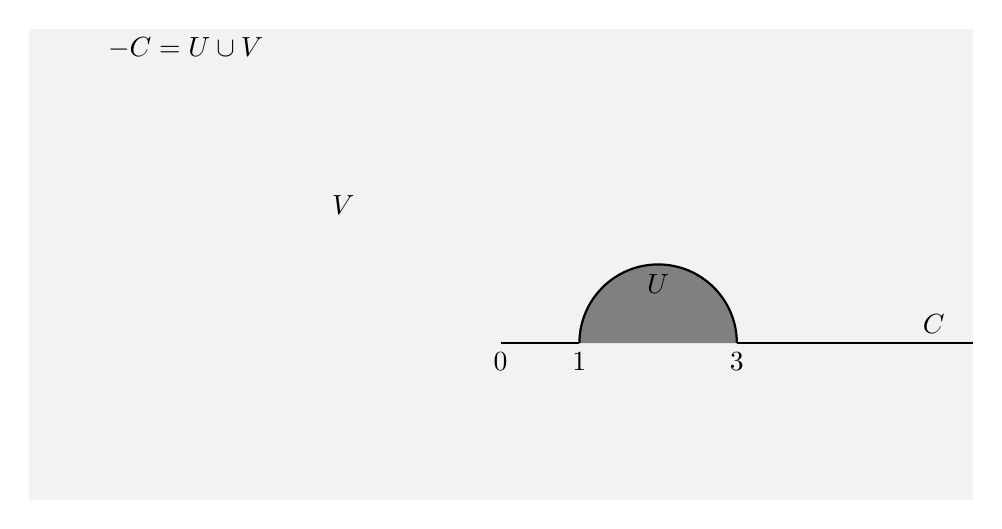
\begin{tikzpicture}
\draw[white, fill=gray!10] (-6,-2) rectangle (6,4);
\draw[shift={(3,0)}, thick, fill=gray!100] (2:0) arc (0:180:1cm);
\draw (2,1) node[below]{$U$} ;
\draw[thick] (0,0) -- (1,0) ;
\draw[thick] (3,0) -- (6,0) ;
\draw (0,0) node[below]{$0$} ;
\draw (-2,2) node[below]{$V$} ;
\draw (3,0) node[below]{$3$} ;
\draw (5.5,0) node[above]{$C$} ;
\draw (1,0) node[below]{$1$} ;
\draw (-4,4) node[below]{$\Cc-C=U\cup V$} ;
\end{tikzpicture}$$
On précisera sur $U$ et sur $V$ l'argument choisi dans la définition du logarithme.}
\reponse{On définit une détermination du logarithme en posant
$$\begin{array}{cccc}
 \ell :& \Cc-L & \longrightarrow & \Cc\\ & z=re^{i\theta} (r>0, 0\leq\theta<2\pi)&\longmapsto& 
 \left\{\begin{array}{l} \textrm{sur } U, \\ \ \ \ \ \ell(z)=\log_\Rr(r)+i(\theta +2\pi).\\
 \textrm{sur } V, \\ \ \ \ \ \ell(z)=\log_\Rr(r)+i\theta\end{array}
 \right.
\end{array}$$
On vérifie que $\ell$ est continue : en particulier sur le disque ouvert de centre $(2,0)$ et de rayon $1$, $\ell$ coïncide avec la fonction $\log +2i\pi$,
qui est continue. 
On vérifie aussi que pour tout $z\in\Cc-L$, $e^{\ell(z)}=z$ : c'est donc une détermination du logarithme sur $\Cc-L$.}
\end{enumerate}
}
